\claude{
\section[When delay reconstruction supports a dimension estimate]{When delay reconstruction supports a dimension estimate}\label{app:theory}
\subsection{Dimension preservation under delay reconstruction}
\cx{When does the dimension measured in a log equal the dimension of the motion that produced it? For a stationary ergodic process, the occupation measure $\mu(A)$ gives the long-run fraction of steps with $s_t\in A$ when the boundary of $A$ has zero measure. Its local dimension at $s$ is}
\begin{equation}
d_{\rm act}=\lim_{\epsilon\to0^+}
\frac{\log\mu(B(s,\epsilon))}{\log\epsilon},
\label{eq:active}
\end{equation}
where $B(s,\epsilon)$ is a ball of radius $\epsilon$ in the state-space metric, taken to be Euclidean for the vector states here. We use a single dimension when the limit exists and is constant $\mu$-almost everywhere. For $r$ independent phases on a smooth invariant torus with regular density, the dimension is $r$.


\begin{proposition}[Preservation of local dimension]
Let $\mu$ have local dimension $d$ at $s$. Suppose $F$ is bi-Lipschitz on the support of $\mu$, meaning $c\|x-y\|\le\|F(x)-F(y)\|\le C\|x-y\|$ for all $x,y$ there and constants $0<c\le C<\infty$. The distribution $F_\#\mu$ of reconstructed points then has local dimension $d$ at $F(s)$.
\end{proposition}
\begin{proof}
For sufficiently small $\epsilon$, the inverse image of $B(F(s),\epsilon)$ is bounded on the support between $B(s,\epsilon/C)$ and $B(s,\epsilon/c)$. Their probabilities bound the pushforward probability. The logarithms of $c$ and $C$ contribute vanishing constants after division by $\log\epsilon$, so both bounds have the same limiting exponent $d$.
\end{proof}
Takens gives conditions under which delays of a scalar observation embed the state of a smooth autonomous system \citep{takens1981detecting}. A smooth embedding of a compact smooth manifold supplies the required distance bounds. Sauer et al.\ extend reconstruction to fractal sets \citep{sauer1991embedology}. Stark and colleagues give embedding results for deterministic and stochastic forcing under assumptions on the dynamics and observations \citep{stark1999delay,stark2003delay}. Applying the proposition requires control of distance distortion on the support being measured.


\subsection{Recurrent, transient, and stochastic regimes}
\cx{An embedding can distinguish states, but a finite record must also revisit their neighborhoods to measure how probability grows with radius. A periodic orbit supplies such visits. A transient can trace a thin curve in a single pass, and a stochastic input can spread nearby observations apart (Figure~\ref{fig:shapes}). In those cases we interpret MG through independent measurements, as in Section~\ref{sec:applied}.}

\begin{figure}[H]
\centering
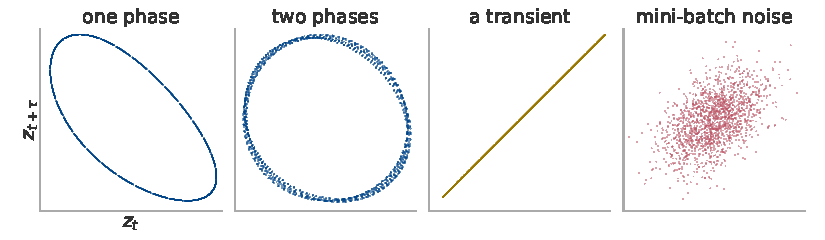
\includegraphics[width=.86\linewidth]{figures/icomp_shapes.pdf}
\caption{Delay reconstructions of periodic, quasiperiodic, transient, and stochastically forced signals. The panels show coordinates $z_t$ and $z_{t+\tau}$.}
\label{fig:shapes}
\end{figure}


\subsection{Computing the pooled estimator}
\cx{We add small independent Gaussian noise (dither) to standardized samples to break ties. Table~\ref{tab:mg-numerics} gives the floors on distances and per-query log-ratio sums. The estimator flags a window when too many distances or sums reach their floor. Forecast sampling and VAE check scheduling discard flagged estimates. Nonfinite or constant records, short windows and too few eligible neighbors yield no estimate.}

\subsection[Changes of scale and offset]{Changes of scale and offset}
\begin{proposition}[Scaling and shifting a record]
For a finite nonconstant record, fixed delay and neighbor settings, and no numerical dither, the MG formula is unchanged by replacing every observation with $ax_t+b$, for any $a\ne0$, provided the estimate is defined.
\end{proposition}
\begin{proof}
\cx{Standardizing $ax_t+b$ multiplies each standardized sample by $\operatorname{sign}(a)$. This preserves all Euclidean distances, temporal exclusions and the distance ratios in Equation~\eqref{eq:mg}.}
\end{proof}
A common positive scale and offset applied to every sample leave the standardized record and its MG unchanged for the same dither. With a negative scale, the estimate has the same distribution under symmetric dither. Finite precision can affect estimates on almost constant records.

\subsection{Pooling and dependence}
\cx{The $-1$ in the numerator corrects bias under a Gamma model with independent local statistics. Queries can share neighbors and eligible observations can remain correlated after temporal exclusion, so finite-sample bias can persist. The implementation retains estimates above $E$.}

\section{Configurations and reproducibility}\label{app:settings}
\cx{Table~\ref{tab:mg-settings} lists the scalar series and window settings used for each experiment. Stride is the distance between window starts. The span rule excludes neighbors within $(E-1)\tau$ time steps. The autocorrelation rule (ACF) expands this interval to the autocorrelation time if longer. Both obey the upper limit shown where applicable.}

\begin{table*}[htbp]
\centering\small
\caption{Scalar records and MG settings.}
\label{tab:mg-settings}
\begin{tabularx}{\linewidth}{@{}l>{\raggedright\arraybackslash}Xrrrrll@{}}
\toprule
Experiment & Observable & $W$ & $E$ & $\tau$ & $k$ & Theiler exclusion & Stride \\
\midrule
Digits head & state-based & 8,000 & 20 & 4 & 20 & span; cap 150 & 3,000 \\
Regression & loss / fixed-example error & 2,048; 8,192 & 16 & 1 & 10 & 100 & first / last \\
Generator & neuron zero & 8,192 & 20 & adaptive & 20 & ACF; cap 320 & 8,192 \\
FORCE transition figure & neuron zero & 4,096 & 20 & 4 & 20 & 156 & 512 \\
CNN / ResNet-18 & parameter norm & 1,000 & 20 & 1 & 20 & span & 500 \\
Text VAE & fixed-set NLL & 512 & 20 & 1 & 20 & 39 & 128 \\
VAE check scheduling & fixed-set NLL & 512 & 20 & 1 & 20 & 39 & 64 \\
Walker2d motion & joint / action scalar & 2,048 & 20 & 8 & 20 & 312 & 1,024 \\
Walker2d selection & action norm & 2,048 & 20 & 8 & 20 & 312 & episode \\
Grokking & parameter norm & 60 & 10 & 1 & 20 & ACF & aligned windows \\
Self-supervised & gradient norm & 1,000 & 20 & 1 & 20 & 19 & final window \\
Spike warning & log loss & 500 & 20 & 1 & 20 & 19 & 50 \\
Forecast selection & single neuron & 2,048 & 20 & adaptive & 20 & ACF; cap 150 & one window \\
MNIST interventions & norm or fixed-set loss & 256 & 10 & 1 & 10 & 19 & candidate updates \\
\bottomrule
\end{tabularx}
\end{table*}

\begin{table}[htbp]
\centering\small
\caption{Noise scale and minimum values used to compute MG.}
\label{tab:mg-numerics}
\begin{tabular}{lr}
\toprule
Quantity & Value \\
\midrule
Standard deviation of added Gaussian noise & $10^{-9}$ \\
Distance floor & $10^{-8}$ \\
Local log-sum floor & $10^{-5}$ \\
Flag if fraction at either floor exceeds & 1\% \\
\bottomrule
\end{tabular}
\end{table}

\begin{table}[htbp]
\centering\small
\caption{Model architectures by experiment.}
\label{tab:architectures}
\begin{tabularx}{\linewidth}{@{}>{\raggedright\arraybackslash}p{.26\linewidth}X@{}}
\toprule
Task & Model \\
\midrule
Digit classifier & Fixed multilayer perceptron with two 64-neuron tanh layers. Train a linear classifier within a fixed parameter subspace. \\
Synthetic generators and forecasting & FORCE-trained recurrent networks with 1,000 neurons for phase recovery and 256 for the periodic-signal and forecast tasks \\
CIFAR-10 interventions & Convolutional neural network (CNN) with ReLU activations and $3\times3$ kernels. Channel counts 16, 32, and 32. Max pooling after the first two layers, then adaptive average pooling and a linear classifier. \\
ResNet transfer & ResNet-18 with a ten-class classifier. Random initialization uses a $3\times3$ input convolution with stride 1 and no max pooling. ImageNet initialization uses a $7\times7$ input convolution with stride 2 and max pooling. \\
Text VAE & 48-dimensional shared embeddings, GRU encoder and decoder with hidden size 64, 16-dimensional Gaussian code \\
Grokking & One-layer transformer, width 128, four 32-dimensional heads, MLP width 512, no layer normalization; full-batch comparison uses a width-500 quadratic perceptron \\
MNIST representation selection & 784--256--256 encoder with batch normalization and ReLU; 256--256--64 projector (one variant outputs 16 coordinates); predictor width 64 in the standard SimSiam/BYOL settings \\
MNIST intervention rules & 196--128--128--10 ReLU MLP; pruning narrows both hidden layers \\
Loss-spike warning & Pre-layer-normalized transformer with two layers, width 64, and four heads \\
Walker2d & Separate 64--64 tanh MLPs for actor and critic; six action outputs \\
\bottomrule
\end{tabularx}
\end{table}

\begin{table}[htbp]
\centering\small
\caption{Classifier intervention and detector settings.}
\label{tab:cnn-protocol}
\begin{tabularx}{\linewidth}{@{}>{\raggedright\arraybackslash}p{.28\linewidth}X@{}}
\toprule
Component & Setting \\
\midrule
\multicolumn{2}{@{}l}{\textbf{CIFAR-10 intervention benchmark}} \\
Small CNN training & 10,000 CIFAR-10 images; 10,000 SGD updates; learning rate 0.02, momentum 0.9, weight decay $5\cdot10^{-4}$, batch 64 with replacement \\
Intervention update & 4,000; pre/post summaries exclude windows that overlap the intervention \\
Interventions & Divide the learning rate by 3, 10, or 100. Freeze the first two convolutions, all layers before the classifier, or all weights except the classifier bias. Prune 50\%, 80\%, or 95\% of weights. \\
Comparison records & Unchanged training or four times the batch size. Two additional records multiply the later part of an unchanged log by 10 or smooth it with a mean over the latest 16 samples. \\
Replication & 4 development and 4 held-out repeats; 10 additional repeats for timing-shift transfer \\
\addlinespace
\multicolumn{2}{@{}l}{\textbf{Detector calibration and comparisons}} \\
Detector & $M=2$, $B=3$, $D_j<-0.08829884$; feature windows ending at or before update 1,500 are excluded \\
Scoring & 5,000 updates after intervention. Each evaluation repeat includes 7 strong intervention types and 4 comparison conditions. \cx{The strong set excludes the threefold learning-rate reduction and freezing the first two convolutions.} \\
Calibration choices & $M\in\{2,3,4\}$, $B\in\{3,4,6\}$. The threshold adds a margin of 0.02 beyond the largest score in the development comparison records. \\
IAAFT surrogates & 2 reordered records per window, 100 iterations. Trimming to match the beginning and end can remove up to 15\% of the window. \\
Entropy features & Permutation order 5, delay 1, stable tie sorting, \cx{normalization by $\log(5!)$}. Sample-entropy template length 2, delay 1, Chebyshev distance, tolerance 0.2 window SDs, no self-matches. \\
CUSUM calibration & Estimate the initial mean and scale on windows ending at updates 2,000--3,500. Use a minimum scale $\max(0.01|\mu_0|,10^{-10})$. Test drift parameters $\{0.25,0.5,1\}$ with threshold margin 0.5. \\
Loss of active channels & Increase the learning rate by a factor of 20, 30, 50, or 100 for one update, 15 for three updates, or 20 for two. Measure inactivity on 500 images \cx{every 250 updates. Require the median inactive fraction in updates 5,000--9,000 to exceed that in $[2{,}000,4{,}000)$ by at least 0.05. Training accuracy below 20\% denotes network-wide failure.} \\
\cx{Training-loss comparison} & \cx{Use the median minibatch loss in each window. With $M=2$ and $B=3$, alarm if $D_j>-0.0590403$.} \\
\addlinespace
\multicolumn{2}{@{}l}{\textbf{Transfer to ResNet-18}} \\
ResNet data and SGD & Full CIFAR-10. Random initialization uses $32\times32$ inputs. ImageNet initialization uses $64\times64$ with ImageNet normalization. Batch 128 without augmentation, learning rate 0.02, momentum 0.9, weight decay $5\cdot10^{-4}$. \\
ResNet update covariance & 3 repeats per initialization type. Each update is compressed to 1,024 coordinates before computing covariance PR. \\
\bottomrule
\end{tabularx}
\end{table}

\begin{table}[htbp]
\centering\small
\caption{Text VAE penalty comparisons and check scheduling.}
\label{tab:vae-protocol}
\begin{tabularx}{\linewidth}{@{}>{\raggedright\arraybackslash}p{.28\linewidth}X@{}}
\toprule
Component & Setting \\
\midrule
Data & 6,000 training and 256 evaluation sentences, 8--24 words before the end-of-sentence marker. Vocabulary of 2,000 tokens. \\
Training & The decoder receives the actual preceding words. Adam learning rate $10^{-3}$, 32 sentences per batch, gradient norm limited to 5, zero dropout. \\
\addlinespace
\multicolumn{2}{@{}l}{\textbf{Penalty comparison}} \\
Penalty conditions & Train to update 1,024 at $\beta=0.01$. Continue from this training state to update 3,072 for each setting. Use $\beta=0.01$, $\beta=1$, or $\beta=1$ with free bits (0.5 nats per coordinate). \\
Recorded reconstruction loss & 16 fixed evaluation sentences per update. Early windows end at updates 512--1,024 and late windows at 2,048--3,072. \\
Code-use measurements & Every 128 updates. For MI, draw 4 codes per sentence from its encoder distribution. For the code-swap test, average the divergence of token predictions in both directions. \\
Comparing code use within a repeat & Loss of code use requires both measurements to fall below half of their low-penalty values. Preservation requires each to retain at least half its early value and double its value under suppression. \\
\addlinespace
\multicolumn{2}{@{}l}{\textbf{Scheduling information checks}} \\
Repeated penalty schedule & After 1,024 initial updates \cx{at $\beta=0.01$}, repeat a 2,048-update schedule three times. Raise the penalty weight $\beta$ from 0 to 1 \cx{over the first 1,024 updates}, then hold it at 1. \\
Loss and recovery labels & Measure MI and code-swap divergence every 64 updates. Divide each by its median from checks 128 updates apart between 512 and 1,024. Loss requires both ratios $\le0.50$ and recovery both $\ge0.65$ for two consecutive checks. \cx{The second check sets the event time. Score events with a full 512 updates left for detection.} \\
\cx{Eligible starting state} & \cx{The early MI and code-swap medians must exceed $0.1$ and $10^{-4}$ nats, respectively. At update 1,024 both ratios must be at least $0.65$.} \\
Check schedules & One initial check; extra budgets 6, 12, 24 \cx{with 12 primary}; at least 128 updates between triggered checks; 1 development and 9 evaluation repeats \\
\cx{Threshold grid} & \cx{$0.025,0.05,0.075,0.1,0.15,0.2,0.3,0.4,0.5,0.7,1,1.5,2,3$. Maximize detections for each method and budget. Break ties by fewer unproductive checks, shorter mean delay, fewer total checks, and a larger threshold, in that order.} \\
\bottomrule
\end{tabularx}
\end{table}

\begin{table}[htbp]
\centering\small
\caption{Walker2d training and evaluation settings.}
\label{tab:walker-protocol}
\begin{tabularx}{\linewidth}{@{}>{\raggedright\arraybackslash}p{.27\linewidth}X@{}}
\toprule
Component & Setting \\
\midrule
\multicolumn{2}{@{}l}{\textbf{Policy training}} \\
Proximal policy optimization (PPO) & Collect 512 steps in each of 8 environments per training round. Minibatch 256, 5 optimization epochs. \\
Optimizer & Learning rate decreases from $3\cdot10^{-5}$ to $3\cdot10^{-6}$. PPO clipping parameter 0.1, KL stopping parameter 0.01, gradient norm limit 0.5. \\
Training objective & Reward discount 0.99, generalized advantage estimation parameter 0.95, entropy weight 0, value-loss weight 0.5. The normalization statistics are fixed. \\
Continued training (fine-tuning) & For each penalty strength, start from the policy saved at 655,360 simulator steps and continue for 1,048,576 steps, summed across environments. \\
\addlinespace
\multicolumn{2}{@{}l}{\textbf{Command smoothing and state repeatability}} \\
Fixed-policy motion records & Discard 512 initial steps and record 4,096. The reference gait uses 152 samples. Its prescribed stride lasts about 152.215 simulator steps. \\
\cx{Reference-gait penalty} & \cx{Compare $\lambda=0$ with $\lambda=3$ at $\sigma^2=38.4774$. The reference advances by $(1+\sqrt{2}/1000)^{-1}$ samples per simulator step. Both policies resume from the same training state.} \\
State and performance criteria & In the reference-gait test, require return error and phase-matched variation ratios $\le0.75$ against training without the reference reward. Require at least eight common complete simulations, at least 90\% of the comparison reward, and at most one extra fall. Baseline return error and variation must be at least 0.02 and 0.001. \\
\addlinespace
\multicolumn{2}{@{}l}{\textbf{Policy choice under actuator shifts}} \\
Candidate policies & Use penalty strengths $\lambda\in\{0,0.25,1,4\}$ and save after 262,144, 524,288, 786,432, and 1,048,576 further steps. Four evaluation repeats. \\
Choice in unperturbed trials & Three episodes per candidate. Discard 256 steps and measure 2,048. Require at least two completed episodes and at least 90\% of the best mean reward in these trials. \\
Fixed policy choice & Use the final policy with $\lambda=0.25$, chosen on a preliminary run, if eligible. Otherwise select the highest unperturbed reward. \\
Perturbed trials & Mix in the previous filtered value with weight $\alpha\in\{0.05,0.1,0.2\}$. Use Gaussian noise of standard deviation $\sigma\in\{0,0.02\}$, with five episodes per condition. \\
\bottomrule
\end{tabularx}
\end{table}

\begin{table}[htbp]
\centering\small
\caption{Grokking runs and the matched-window analysis.}
\label{tab:grokking-protocol}
\begin{tabularx}{\linewidth}{@{}>{\raggedright\arraybackslash}p{.26\linewidth}X@{}}
\toprule
Component & Setting \\
\midrule
Modular addition & Modulus 113; training fraction 0.30; weight decay 1.0; 20,000 optimizer updates; 3 regularized runs \\
Permutation composition & $S_5$; training fraction 0.50; weight decay 0.2; 30,000 optimizer updates \cx{over 15,000 loop iterations with two updates per iteration}; 1 regularized run \\
Transformer optimization & AdamW at $10^{-3}$, \cx{$(\beta_1,\beta_2)=(0.9,0.98)$}, batch 256, float64 \\
Comparison runs & One run with zero weight decay per task. The perceptron uses half the modulo-97 addition pairs and full-batch gradient descent on squared error. \\
Matched windows & 60 log samples centered on each covariance estimate. $E\in\{4,6,10\}$, $\tau\in\{1,2,4\}$, $k\in\{5,20\}$. Exclusion uses the span or autocorrelation time. \\
\bottomrule
\end{tabularx}
\end{table}


\paragraph{Exact adaptive rules.}
For centered samples $z_t$, define $a(\ell)=\sum_{t=1}^{W-\ell}z_tz_{t+\ell}/\sum_{t=1}^Wz_t^2$. The autocorrelation time $t_a$ is the first lag with $a(\ell)<e^{-1}$, or $W$ if none exists. The autocorrelation routine returns zero when the sample standard deviation is below $10^{-12}$. We compute the adaptive lag from the original window and the autocorrelation exclusion from the standardized, dithered window. The adaptive generator uses
\[
\begin{aligned}
\tau_0&=\max(1,\operatorname{round}(t_a/4)),\\
\tau&=\min\{\tau_0,\max(1,\lfloor W/[8(E-1)]\rfloor)\}.
\end{aligned}
\]
The implementation uses nearest-even rounding. The span limit keeps most samples available as starting points for delay vectors. The search requests $k+2T+1$ candidates to allow for temporal exclusions and the query itself, so limiting $T$ bounds this work. Theiler settings resolve to $T=\min(T_{\max},T_0)$, where $T_0=(E-1)\tau$ for the embedding rule and $T_0=\max((E-1)\tau,t_a)$ for the autocorrelation rule. Explicit choices of $T$ obey the same upper limit. When $T_{\max}<(E-1)\tau$, the resolved exclusion is shorter than the delay span. Eligible delay vectors can still overlap or be correlated.


\paragraph{Window length and recurrence requirements.}
For $T>0$, retaining $k$ eligible neighbors for every query requires $n\ge 2T+k+1$, or $W\ge(E-1)\tau+2T+k+1$. The shared code also checks the input length before reconstruction. It needs at least $E\tau+20$ samples for a fixed lag and $E+20$ for an adaptive lag. For dimension estimation the window must also cover repeated visits within a regime. For detection, longer windows smooth estimates and delay the response.

\paragraph{What is compared within each repeat.}
\cx{Within each repeat, CNN and VAE conditions share a starting model, generator tasks share initial weights, and Walker2d rules choose among the same policies. Resampling for intervals keeps each repeat's measurements together.}

\section[Dimension tests and recurrent generators]{Dimension tests and recurrent generators}\label{app:controlled}
\subsection[Oscillations in the diagonal matrix and digit classifier]{Oscillations in the diagonal matrix and digit classifier}
\cx{The Frobenius norm combines all the entries of the matrix by summing their squares and taking the square root. A single oscillating entry records only its own rhythm. Comparing the two logs shows which oscillations an estimate can recover from the same system (Table~\ref{tab:matrix-observations}).}

\begin{table}[!htbp]
\centering\small
\caption{\cx{Oscillating diagonal matrix. Median MG over four runs per dimension. MAE is the mean absolute error against the prescribed dimensions.}}
\label{tab:matrix-observations}
\begin{tabular}{@{}lrrrrr@{}}
\toprule
 & \multicolumn{4}{c}{\cx{Independent oscillations}} & \\
\cmidrule(lr){2-5}
\cx{Recorded quantity} & \cx{1} & \cx{3} & \cx{5} & \cx{8} & \cx{MAE} \\
\midrule
\cx{Matrix norm} & \cx{1.14} & \cx{3.48} & \cx{5.29} & \cx{7.83} & \cx{0.27} \\
\cx{One oscillating entry} & \cx{1.14} & \cx{1.12} & \cx{1.14} & \cx{1.12} & \cx{3.19} \\
\bottomrule
\end{tabular}
\end{table}

\cx{For the classifier, the loss weights set the frequencies, while the optimizer determines how far the weights move in each direction. We use the observed weight covariance PR to assess which scalar logs capture that motion (Table~\ref{tab:synthetic-errors}).}


\begin{table}[htbp]
\centering\small
\setlength{\tabcolsep}{2.5pt}
\caption{\cx{Digit classifier. Error against weight covariance PR, averaged over four held-out ranks and four repeats per rank.}}
\label{tab:synthetic-errors}
\begin{tabular}{lr}
\toprule
Recorded quantity & Mean absolute error \\
\midrule
Parameter norm & 0.57 \\
Loss on fixed examples & 0.59 \\
Fixed parameter projection & 0.62 \\
Gradient norm & 1.70 \\
\midrule
\cx{Pooled over all 10 usable quantities} & \cx{0.90} \\
\bottomrule
\end{tabular}
\end{table}

We use the handwritten-digit data distributed with scikit-learn \citep{pedregosa2011scikit}. We train and freeze a multilayer perceptron that extracts features, then train a linear classifier whose weights move within a fixed affine subspace. We randomly assign each training example to a subset before training the classifier. All examples in subset $i$ share the time-dependent coefficient $w_i(t)$ in the cross-entropy loss
\[
w_i(t)=\max\!\left\{0.05,1+0.8\sum_{j=1}^r G_{ji}\sum_{\ell=1}^r A_{j\ell}\sin(2\pi f_\ell t+\phi_\ell)\right\}.
\]
\cx{Each column of $G$ sets the coefficients for an image subset. The mixing matrix $A$ balances the effect of the oscillations on early weight updates. We draw phases uniformly on $[0,2\pi)$. The frequencies depend on $p_j$, the $j$th prime, as follows.}
\[
\begin{aligned}
 f_1 &= \sqrt{2}/16 && (r=1),\\
 f_j &= 2^{a_j}/16,\quad
 a_j=0.03+0.94\,\frac{b_j-\min b}{\max b-\min b},\quad
 b_j=\operatorname{frac}(\sqrt{p_j}) && (r>1).
\end{aligned}
\]

\cx{We compute the gradient norm from the full unweighted training loss in subspace coordinates. At zero learning rate fresh minibatches can still change the loss, while accuracy on fixed examples can take too few distinct values for MG. Table~\ref{tab:learning-oscillator-settings} gives the training settings.}

\begin{table}[!htbp]
\centering\small
\caption{\cx{Training settings for the digit classifier and regression.}}
\label{tab:learning-oscillator-settings}
\begin{tabularx}{\linewidth}{@{}>{\raggedright\arraybackslash}p{.38\linewidth}>{\raggedright\arraybackslash}X@{}}
\toprule
Parameter & Setting \\
\midrule
\multicolumn{2}{@{}l}{\textbf{Digit classifier}} \\
Fixed image subsets / preconditioned step size & 12 / 0.15 \\
Development ranks / repeats & $\{2,4,6\}$ / 3 \\
Evaluation ranks / repeats & $\{1,3,5,8\}$ / 4 \\
\addlinespace
\multicolumn{2}{@{}l}{\textbf{Dense regression}} \\
Examples / weights & 256 / 32 \\
Initial learning rate / momentum & 1 / 1 \\
Damping update / changed momentum / affected modes & 8,192 / 0.98 / 2 of 4 \\
Start of final window & 12,288 \\
\bottomrule
\end{tabularx}
\end{table}

\subsection[Oscillations in linear regression]{Oscillations in linear regression}
The squared-loss Hessian is $H=X^\top X/N$, where $X$ has full column rank and $N$ rows. The weight error is the current weight vector minus the optimal one. For each of $r$ distinct Hessian eigenvalues, we initialize an error component along one eigenvector in that eigenspace. The projection onto that eigenvector is $q_{j,t}$ for mode $j$ at step $t$. With learning rate and momentum coefficient both equal to one,
\[
q_{j,t+1}=2\cos(\omega_j)q_{j,t}-q_{j,t-1},
\qquad \lambda_j=2(1-\cos\omega_j).
\]
Here $\omega_j$ is the angular frequency and $\lambda_j$ is the Hessian eigenvalue for mode $j$. We choose frequencies that produce $r$ independent phases and rotate the eigenbasis so all original weight coordinates vary. We also record prediction error on one fixed test input.

\begin{table}[h]
\centering\small
\caption{Median MG in regression with $r$ known modes.}
\begin{tabular}{rrrr}
\toprule
Modes $r$ & \multicolumn{2}{c}{Training loss} & Fixed-input error \\
\cmidrule(lr){2-3}
 & 2,048 samples & 8,192 samples & 8,192 samples \\
\midrule
1 & 0.90 & 1.12 & 1.01 \\
2 & 2.39 & 2.57 & 2.55 \\
4 & 3.71 & 4.99 & 4.11 \\
6 & 5.88 & 7.00 & 4.98 \\
\bottomrule
\end{tabular}

\end{table}

\cx{Estimator settings are fixed across modes. We use the last window of each stationary run, and the first and last windows for the damping comparison. Rotating the eigenbasis leaves the full-batch loss and its MG unchanged across repeats but changes the fixed-input error (Table~\ref{tab:regression_variation}). With momentum below one, roundoff can dominate a nearly constant loss after standardization.}

\begin{table}[h]
\centering\small
\caption{Median MG before and after damping, across three runs. Brackets give the range.}
\label{tab:regression_variation}
\begin{tabular}{lrr}
\toprule
Recorded quantity & Before damping & After damping \\
\midrule
Training loss & 4.971 & 2.563 \\
Fixed-input error & 4.154 [3.601, 4.206] & 2.634 [1.996, 2.681] \\
\bottomrule
\end{tabular}

\end{table}

\subsection{Learned autonomous generators}
\cx{The recurrent generator feeds its output back into the state update,}
\[
\begin{aligned}
\boldsymbol h_{t+1}&=0.9\boldsymbol h_t+
0.1(J\tanh\boldsymbol h_t+U\boldsymbol z_t),\\
\boldsymbol z_t&=A^\top\tanh\boldsymbol h_t.
\end{aligned}
\]
\cx{Here $J$ couples neurons, $U$ feeds back the output, and $A$ maps activations $\tanh\boldsymbol h_t$ to that output. Gain $g$ sets the initial standard deviation of $J$'s entries to $g/\sqrt n$ for $n$ neurons (Table~\ref{tab:architectures}). We take median MG over disjoint windows of the same neuron's activation and repeat for other neurons. For comparison we measure covariance PR from all activations and identify spectral peaks in the summed output (Table~\ref{tab:controlled-settings}).}


\begin{table}[htbp]
\centering\small
\caption{Phase structure in learned generators. Entries show mean $\pm$ standard deviation across five runs. MG uses one neuron and PR uses all activations.}
\label{tab:generator_phases}
\begin{tabular}{lrrr}
\toprule
Task & Phases & MG & Covariance PR \\
\midrule
T1 & 1 & \cx{$1.14 \pm 0.03$} & \cx{$1.66 \pm 0.08$} \\
T2 & 2 & \cx{$2.80 \pm 0.09$} & \cx{$2.98 \pm 0.07$} \\
T3 & 3 & \cx{$6.37 \pm 1.29$} & \cx{$4.36 \pm 0.10$} \\
T4 & 4 & \cx{$5.62 \pm 0.84$} & \cx{$5.75 \pm 0.08$} \\
H2 & 1 & \cx{$1.05 \pm 0.18$} & \cx{$2.94 \pm 0.09$} \\
H4 & 1 & \cx{$1.151 \pm 0.001$} & \cx{$5.33 \pm 0.11$} \\
M4 & 2 & \cx{$3.46 \pm 0.24$} & \cx{$5.67 \pm 0.11$} \\
\bottomrule
\end{tabular}

\end{table}

\begin{table}[!htbp]
\centering\small
\caption{\cx{Training and measurement settings for the recurrent generators.}}
\label{tab:controlled-settings}
\begin{tabularx}{\linewidth}{@{}>{\raggedright\arraybackslash}p{.38\linewidth}>{\raggedright\arraybackslash}X@{}}
\toprule
Parameter & Setting \\
\midrule
\multicolumn{2}{@{}l}{\textbf{Learned generators}} \\
T1--T4 frequencies, relative to scale & $1,\sqrt{2},\sqrt{3},\sqrt{5}$ \\
H2/H4 and M4 frequencies, relative to scale & Integer harmonics (H2/H4), $1,2,\sqrt{2},2\sqrt{2}$ (M4) \\
Frequency scale / amplitude per tone / phase & $(10\pi)^{-1}$ / $1.2/\sqrt{q}$ for $q$ tones / uniform on $[0,2\pi)$ \\
Gain / FORCE steps with recursive least squares / repeats per task & 1.2 / 100,000 / 5 \\
Initial fixed-weight steps discarded / samples kept & 5,000 / 32,768 \\
\cx{Simulation step / MG windows per neuron} & \cx{0.1 / 4} \\
\cx{Sampling for full-state PR} & \cx{Every fourth activation vector} \\
\cx{Minimum spectral peak power} & \cx{5\% of nonzero-frequency power in summed output} \\
Output fidelity (Hann window) & $\ge80\%$ of nonzero-frequency power within 3\% of the prescribed frequency, per output \\
Lyapunov exponents / first steps used / inclusion threshold & 12 largest / 16,384 / $\ge-0.02$ per unit time \\
\cx{QR factorization interval / initial propagation discarded (steps)} & \cx{10 / 1,000} \\
Noise test (first samples / neurons / tasks) & $\{4{,}096,8{,}192\}$ / 3 / H4, M4, T4 \\
Gaussian noise SD relative to observed SD & $\{0,0.01,0.05\}$ \\
\addlinespace
\multicolumn{2}{@{}l}{\textbf{Transition to periodic motion}} \\
Gain / FORCE steps & 1.5 / 40,000 \\
\cx{Largest and next-largest Lyapunov exponents} & \cx{$|\lambda_1|<0.005$, $\lambda_2<-0.005$} \\
\cx{Output and state-return errors} & \cx{Normalized root mean squared error $<0.1$ for each} \\
Initial fixed-weight steps discarded / samples kept & 2,000 / 8,192 \\
\bottomrule
\end{tabularx}\par\smallskip
\begin{tabularx}{\linewidth}{@{}>{\raggedright\arraybackslash}Xrrr@{}}
\toprule
\multicolumn{4}{@{}l}{\textbf{Resolved settings for four-frequency generator logs}} \\
\midrule
Task & $t_a$ & $\tau$ & $T$ \\
\midrule
H4 & 21--29 & 5--7 & 95--133 \\
M4 & 28--40 & 7--10 & 133--190 \\
T4 & 32--40 & 8--10 & 152--190 \\
\bottomrule
\end{tabularx}
\end{table}

\cx{Among generators with equally many output frequencies, MG rises with the number of independent phases in every matched repeat. All networks reproduce their prescribed frequencies (Table~\ref{tab:controlled-settings}).}

\cx{We estimate finite-time Lyapunov exponents by propagating small state perturbations through successive update Jacobians with weights fixed. Periodic $QR$ factorization restores orthonormal perturbations. After the initial transient, summing $\log|R_{ii}|$ and dividing by elapsed time gives the exponent for direction $i$. The number of exponents at or above the cutoff usually matches the number of independent phases, although some harmonic runs have weakly contracting directions close to the cutoff (Table~\ref{tab:controlled-settings}).}

\cx{Low observation noise preserves the ordering by phase structure. At higher noise the ordering becomes inconsistent.}

The prescribed output for the periodic-signal experiment is $(\sin\theta,\tfrac12\sin 2\theta)$, with phase $\theta$ increasing at a constant rate. \cx{We check whether the leading Lyapunov exponent is near zero while the remaining directions contract. The output must also match the prescribed signal after phase alignment, and the hidden state must return close to its starting value after a period (Table~\ref{tab:controlled-settings}). For the latter check we interpolate the shifted states and divide their mean squared return error by total hidden-state variance before taking the square root.}

\begin{table}[htbp]
\centering\small
\caption{Transition to periodic motion during FORCE training.}
\label{tab:force-outcome}
\begin{tabular}{lr}
\toprule
Measure & Result \\
\midrule
Single-neuron MG before training & 3.56--5.07 \\
Single-neuron MG after training & 1.08--1.13 \\
Runs passing the test for stable periodic motion & 4/5 \\
\bottomrule
\end{tabular}
\end{table}

\section{Applied training procedures and full comparisons}\label{app:applied}
\subsection{CNN and ResNet interventions}
\cx{We compare windows entirely before and after each intervention, then take median changes across repeats. Freezing usually lowers both MG and update PR. After moderate pruning they move in opposite directions (Table~\ref{tab:cnn-graded}).}

Freezing reinitializes the optimizer in the small CNN. Pruning reapplies its weight mask after each update. The rescaled and smoothed records use logs from unchanged training.

To test whether the power spectrum accounts for the observed changes, we use the iterative amplitude-adjusted Fourier transform (IAAFT) \citep{schreiber1996improved}. We trim segment ends to reduce jumps across the Fourier boundary, then reorder the retained values with IAAFT to approximately preserve their power spectrum. Table~\ref{tab:cnn-separation} compares separation using the area under the receiver operating characteristic curve (AUC). MG separates interventions less clearly on the reordered records.

\begin{table*}[t]
\centering\small
\caption{Changes in CNN weight motion across four repeats.}
\label{tab:cnn-graded}
\begin{tabular}{lrrrr}
\toprule
Condition & \multicolumn{2}{c}{MG@weight norm} & Update PR change & Weights updated \\
\cmidrule(lr){2-3}
 & After & Change & & \\
\midrule
\multicolumn{5}{l}{\textbf{Comparison conditions}} \\
No intervention & 4.32 & +0.4\% & +40.3\% & 100.00\% \\
Batch $\times4$ & 4.85 & +12.8\% & -7.3\% & 100.00\% \\
Rescale the log by 10 & 4.32 & +0.4\% & +40.3\% & 100.00\% \\
Smoothed log & 4.44 & +3.3\% & +40.3\% & 100.00\% \\
\addlinespace
\multicolumn{5}{l}{\textbf{Learning-rate reductions}} \\
Divide by 3 & 4.35 & +0.9\% & -5.4\% & 100.00\% \\
Divide by 10 & 3.95 & -8.3\% & -21.6\% & 100.00\% \\
Divide by 100 & 3.85 & -11.5\% & -20.9\% & 100.00\% \\
\addlinespace
\multicolumn{5}{l}{\textbf{Freezing}} \\
Freeze first two convolutions & 4.27 & -1.8\% & -13.6\% & 65.31\% \\
Train only the final classifier & 3.51 & -18.5\% & -43.5\% & 2.25\% \\
Train only its bias terms & 3.58 & -16.7\% & -68.4\% & 0.07\% \\
\addlinespace
\multicolumn{5}{l}{\textbf{Pruning}} \\
Prune 50\% & 3.80 & -12.7\% & +14.7\% & 50.30\% \\
Prune 80\% & 3.59 & -17.5\% & -10.3\% & 20.48\% \\
Prune 95\% & 3.79 & -11.5\% & -45.3\% & 5.55\% \\
\bottomrule
\end{tabular}

\par\smallskip
\begin{tabular}{@{}lr@{}}
Median MG before intervention (all conditions) & 4.31 \\
Spearman correlation of MG and PR changes & 0.59 \\
\end{tabular}
\end{table*}

\begin{table}[t]
\centering\small
\caption{Separation from unchanged and larger-batch CNN training.}
\label{tab:cnn-separation}
\begingroup
\begin{tabular}{lr}
\toprule
Statistic & AUC \\
\midrule
MG & 0.93 \\
MG (IAAFT surrogates) & 0.68 \\
Relative detrended standard deviation & 0.57 \\
Trend crossings & 0.56 \\
Correlation of successive residuals & 0.48 \\
\bottomrule
\end{tabular}
\endgroup
\end{table}

\cx{For window statistic $m_j$ ($\MG$ for the MG detector), the relative change from the previous $B$ windows to the latest $M$ is}
\begin{equation}
D_j=\frac{\median(m_{j-M+1},\ldots,m_j)}
{\median(m_{j-M-B+1},\ldots,m_{j-M})}-1.
\label{eq:detector}
\end{equation}
The rule raises an alarm when $-sD_j>\delta$, where $s=1$ for a drop and $s=-1$ for a rise. A comparison is skipped if either block contains a nonfinite score or the earlier median has magnitude at most $10^{-12}$. MG uses $s=1$. On development runs we select the rule with the most detections, using shorter delay to resolve ties. The threshold margin is added to the largest score on development comparison records. An intervention is detected when the first alarm falls within the scoring interval after it. Alarms at or before the intervention are premature. Table~\ref{tab:detectors} reports how many comparison records raised at least one alarm. All conditions use the same evaluation repeats.

\subsection[Comparing scalar detection statistics]{Comparing scalar detection statistics}\label{app:baselines}
We compute comparison statistics on the same weight-norm records. Permutation entropy measures the variety of local orderings~\citep{bandt2002permutation}. Sample entropy measures how often similar short sequences recur~\citep{richman2000physiological}. Normalized increments divide the mean absolute change between adjacent samples by the window standard deviation plus $10^{-12}$. Trend crossings are sign changes in the residuals $r_1,\ldots,r_W$ after subtracting a fitted line. The lag-1 Pearson correlation compares $(r_1,\ldots,r_{W-1})$ with $(r_2,\ldots,r_W)$. Relative detrended standard deviation divides the residual standard deviation by the magnitude of the original window mean plus $10^{-12}$. Spectral entropy measures how broadly power is distributed across frequencies after detrending. We also test a one-sided cumulative sum (CUSUM) rule~\citep{page1954continuous} that accumulates deviations from an earlier baseline. All statistics use the same run split, event definition, and detector search.


\begin{table}[!htbp]
\centering\small
\caption{Detection of strong interventions in the CIFAR-10 classifier. Delay is the median number of updates among detections.}
\label{tab:detectors}
\scriptsize\setlength{\tabcolsep}{2pt}
\begin{tabularx}{\linewidth}{@{}>{\raggedright\arraybackslash}Xrrr@{}}
\toprule
Statistic & Detections & False positives & Delay \\
\midrule
Normalized increments & 28/28 & 0/16 & 1,500 \\
Sample entropy & 28/28 & 4/16 & 1,500 \\
Permutation entropy & 28/28 & 7/16 & 1,500 \\
Relative detrended standard deviation & 28/28 & 10/16 & 500 \\
Absolute increments & 27/28 & 0/16 & 500 \\
MG & 27/28 & 0/16 & 1,000 \\
Trend crossings & 15/28 & 5/16 & 1,000 \\
Window mean & 4/28 & 0/16 & 1,000 \\
Spectral entropy & 4/28 & 2/16 & 2,750 \\
Correlation of successive residuals & 0/28 & 0/16 & --- \\
\bottomrule
\end{tabularx}

\end{table}

\begin{table}[!htbp]
\centering\small
\caption{False alarms by comparison condition.}
\label{tab:baseline_references}
\scriptsize\setlength{\tabcolsep}{2pt}
\begin{tabular}{lrrrr}
\toprule
Statistic & Unchanged & Batch $\times4$ & Rescaled & Smoothed \\
\midrule
Normalized increments & 0 & 0 & 0 & 0 \\
Sample entropy & 1 & 0 & 1 & 2 \\
Permutation entropy & 3 & 0 & 3 & 1 \\
Relative detrended standard deviation & 2 & 2 & 4 & 2 \\
Absolute increments & 0 & 0 & 0 & 0 \\
MG & 0 & 0 & 0 & 0 \\
Trend crossings & 1 & 2 & 1 & 1 \\
Window mean & 0 & 0 & 0 & 0 \\
Spectral entropy & 0 & 2 & 0 & 0 \\
Correlation of successive residuals & 0 & 0 & 0 & 0 \\
\bottomrule
\end{tabular}

\end{table}

\cx{Table~\ref{tab:baseline_rules} gives the fitted directions and thresholds. Both detection rules use the same window statistics.}

CUSUM estimates the baseline mean $\mu_0$ and scale $\sigma_0$ from the initial windows (Table~\ref{tab:cnn-protocol}). After this baseline period, it starts at $C_0=0$ and updates $C_j=\max\{0,C_{j-1}+s(\mu_0-m_j)/\sigma_0-\kappa\}$. The sign $s$ sets the direction and $\kappa$ sets the tolerated drift. An alarm occurs when $C_j$ exceeds the threshold $h$. We choose the alarm direction separately for CUSUM and median comparison on development runs.

\begin{table}[!htbp]
\centering\small
\caption{Detector settings chosen on development runs.}
\label{tab:baseline_rules}
\begin{tabular}{lrrrrrrr}
\toprule
Statistic & \multicolumn{4}{c}{Median comparison} & \multicolumn{3}{c}{Cumulative sum} \\
\cmidrule(lr){2-5}\cmidrule(lr){6-8}
 & $M$ & $B$ & Sign $s$ & Threshold $\delta$ & \cx{Sign $s$} & Drift $\kappa$ & Threshold $h$ \\
\midrule
Normalized increments & 4 & 4 & -1 & 0.0289438 & \cx{$-1$} & 0.25 & 5.90329 \\
Sample entropy & 2 & 3 & -1 & 0.186699 & \cx{$-1$} & 0.25 & 9.86063 \\
Permutation entropy & 2 & 6 & -1 & 0.339038 & \cx{$-1$} & 1.0 & 7.79449 \\
\cx{Relative} detrended standard deviation & 2 & 3 & -1 & 0.305439 & \cx{$-1$} & 0.25 & 0.5 \\
Absolute increments & 2 & 3 & 1 & 0.338305 & \cx{$+1$} & 1.0 & 19.7929 \\
MG & 2 & 3 & 1 & 0.0882988 & \cx{$+1$} & 0.25 & 44.3109 \\
Trend crossings & 2 & 4 & 1 & 0.662857 & \cx{$+1$} & 0.5 & 2.31626 \\
Window mean & 2 & 3 & 1 & 0.02 & \cx{$+1$} & 0.25 & 0.5 \\
Spectral entropy & 3 & 3 & -1 & 1.29961 & \cx{$+1$} & 0.25 & 6.74364 \\
\cx{Detrended} lag-one correlation & 2 & 3 & 1 & 0.0238814 & \cx{$+1$} & 0.25 & 0.653369 \\
\bottomrule
\end{tabular}

\end{table}

\begin{table}[!htbp]
\centering\scriptsize\setlength{\tabcolsep}{2pt}
\caption{CNN intervention detection using cumulative sums. Delay is the median among detected interventions.}
\label{tab:cusum}
\begin{tabular}{lrrr}
\toprule
Statistic & Detections & False positives & Delay (updates) \\
\midrule
\cx{Relative} detrended standard deviation & 28/28 & 4/16 & 500 \\
Normalized increments & 28/28 & 4/16 & 1,000 \\
Permutation entropy & 28/28 & 4/16 & 1,000 \\
Sample entropy & 28/28 & 4/16 & 1,250 \\
Absolute increments & 27/28 & 12/16 & 2,500 \\
MG & 17/28 & 0/16 & 3,500 \\
Trend crossings & 13/28 & 3/16 & 1,000 \\
Spectral entropy & 5/28 & 1/16 & 500 \\
\cx{Detrended} lag-one correlation & 1/28 & 0/16 & 500 \\
Window mean & 0/28 & 0/16 & --- \\
\bottomrule
\end{tabular}

\end{table}

\cx{Normalized increments detect all strong interventions with median comparison. Under CUSUM, they also raise false alarms (Tables~\ref{tab:detectors} and~\ref{tab:cusum}).}

\begin{table}[!htbp]
\centering\small
\caption{CNN detections by time allowed after intervention. \cx{Rules needing eight windows can first score at update 5,500, a delay of 1,500 updates.}}
\label{tab:horizons}
\begin{tabular}{lrrrrr}
\toprule
Statistic & \multicolumn{4}{c}{Detection within this many updates} & False alarms \\
\cmidrule(lr){2-5}
 & 500 & 1,000 & 2,000 & 5,000 & \\
\midrule
Normalized increments & 0/28 & 0/28 & 21/28 & 28/28 & 0/16 \\
Sample entropy & 8/28 & 13/28 & 27/28 & 28/28 & 4/16 \\
Permutation entropy & 0/28 & 0/28 & 23/28 & 28/28 & 7/16 \\
Relative detrended standard deviation & 25/28 & 27/28 & 27/28 & 28/28 & 10/16 \\
Absolute increments & 15/28 & 16/28 & 26/28 & 27/28 & 0/16 \\
MG & 8/28 & 16/28 & 22/28 & 27/28 & 0/16 \\
Trend crossings & 0/28 & 15/28 & 15/28 & 15/28 & 5/16 \\
Window mean & 0/28 & 4/28 & 4/28 & 4/28 & 0/16 \\
Spectral entropy & 0/28 & 0/28 & 0/28 & 4/28 & 2/16 \\
Correlation of successive residuals & 0/28 & 0/28 & 0/28 & 0/28 & 0/16 \\
\bottomrule
\end{tabular}

\end{table}

\cx{Rules that compare longer blocks cannot signal until enough windows have accumulated. This delay explains some missed early detections in Table~\ref{tab:horizons}. With intervention times shifted, we distinguish premature alarms in intervention runs from alarms during unchanged training (Table~\ref{tab:detector-transfer}).}

\begin{table}[!htbp]
\centering\small
\caption{Detector performance at shifted intervention times.}
\label{tab:detector-transfer}
\begingroup
\begin{tabular}{lrrr}
\toprule
Feature & Detected & Alarms on unchanged runs & Premature alarms \\
\midrule
Absolute increments & 30/30 & 0/10 & 0/30 \\
Normalized increments & 29/30 & 2/10 & 0/30 \\
MG & 19/30 & 5/10 & 6/30 \\
\bottomrule
\end{tabular}
\endgroup
\end{table}

\paragraph{Transfer to ResNet-18.}
\cx{We match repeats across random and ImageNet initialization. To estimate update PR, CountSketch} \citep{charikar2002finding} \cx{assigns each update coordinate a random bin and sign. We sum signed entries in each bin and compute PR of the compressed updates' covariance. The transferred detector responds to freezing but misses pruning and learning-rate reductions. Layer norms and random projections produce false alarms.}

\begin{table}[!htbp]
\centering\small
\caption{ResNet-18 feature-extractor freezing.}
\label{tab:resnet-freeze}
\begin{tabular}{lrrr}
\toprule
Initialization & Median MG change & Freeze detections & False alarms \\
\midrule
Random & $-27.6\%$ & 3/3 & 0/12 \\
ImageNet & $-30.8\%$ & 3/3 & 0/12 \\
\bottomrule
\end{tabular}
\end{table}

\subsection[Loss of active ReLU channels]{Loss of active ReLU channels}
A ReLU channel is inactive on a set of images if its output is zero for every image. We test whether the transferred detector flags a rise in the fraction of inactive channels after a brief increase in the learning rate (Table~\ref{tab:cnn-protocol}). We exclude runs with network-wide failure from detection scoring. Runs without channel loss and transformed logs from unchanged training serve as comparisons (Table~\ref{tab:relu-channel-loss}).

\begin{table}[!htbp]
\centering\small
\caption{Detection of newly inactive ReLU channels.}
\label{tab:relu-channel-loss}
\begin{tabularx}{.94\linewidth}{@{}>{\raggedright\arraybackslash}Xrrr@{}}
\toprule
\multicolumn{4}{@{}l}{\textbf{(a) Evaluation records}} \\
\midrule
Record type & Available & Excluded & Scored \\
\midrule
Training runs & 42 & 2 & 40 \\
\quad With channel loss & 23 & 2 & 21 \\
\quad Without channel loss & 19 & 0 & 19 \\
Transformed logs from unchanged training & 12 & 0 & 12 \\
\bottomrule
\end{tabularx}\par\smallskip
\begin{tabularx}{.94\linewidth}{@{}>{\raggedright\arraybackslash}Xrr@{}}
\toprule
\multicolumn{3}{@{}l}{\textbf{(b) Detection results}} \\
\midrule
Statistic & Detections / 21 & False alarms / 31 \\
\midrule
Training-loss comparison & 21 & 8 \\
Relative detrended standard deviation & 21 & 25 \\
Trend crossings & 19 & 7 \\
MG & 12 & 12 \\
Correlation of successive residuals & 0 & 0 \\
\bottomrule
\end{tabularx}
\end{table}
MG can move in opposite directions for channel loss and network-wide failure. Trend crossings detect more channel losses than MG and raise fewer false alarms.

\subsection[Measuring information in the text VAE]{Measuring information in the text VAE}\label{app:vae-information}
Within each repeat, the three training conditions share starting weights, optimizer state, batches, and Gaussian draws. For the batch-average KL divergence $K_j$ of code coordinate $j$, the penalty is $\beta\sum_j K_j$ without free bits and $\beta\sum_j\max(K_j,\lambda)$ with free bits (Table~\ref{tab:vae-protocol}). We log per-token loss on fixed evaluation sentences, reusing the Gaussian draws for their codes.

For $N$ evaluation sentences and $S$ code draws $z_{i\ell}$ from each encoder density $q(z\mid x_i)$, we estimate $I(X;Z)$ for a uniformly chosen sentence by
\begin{equation}
\widehat I(X;Z)=\frac{1}{NS}\sum_{i=1}^N\sum_{\ell=1}^S
\log\frac{q(z_{i\ell}\mid x_i)}{N^{-1}\sum_{j=1}^N q(z_{i\ell}\mid x_j)}.
\label{eq:vae-mi}
\end{equation}
\cx{Natural logarithms give nats. For the decoder test, we shift encoder distributions by one sentence, keeping preceding words and Gaussian draws fixed. We average KL divergence in both directions between the original and reassigned predictions, then average over tokens.}


\begin{table}[htbp]
\centering\small
\caption{\cx{Ratios of median MG over the final VAE evaluation windows, computed within each repeat.}}
\label{tab:vae-mg-ratios}
\begin{tabularx}{\linewidth}{@{}>{\raggedright\arraybackslash}Xrr@{}}
\toprule
Conditions (first / second) & Median ratio & 95\% interval \\
\midrule
Higher penalty / lower penalty & $0.517$ & $[0.480,0.542]$ \\
Higher penalty with free bits / higher penalty alone & $1.286$ & $[1.179,1.418]$ \\
\bottomrule
\end{tabularx}
\end{table}

\begin{table}[!htbp]
\centering\small
\caption{Code-use measurements and MG in the final evaluation interval.}
\label{tab:vae-final}
\begin{tabular}{lrrr}
\toprule
Penalty condition & MI (nats) & \cx{Decoder sensitivity (nats)} & MG \\
\midrule
Lower penalty & 5.545 & 2.087 & 8.129 \\
Higher penalty & 0.327 & 0.021 & 4.172 \\
Higher penalty with free bits & 3.934 & 0.599 & 5.491 \\
\bottomrule
\end{tabular}

\end{table}

\cx{Within a run, each final value is the median over the interval in Table~\ref{tab:vae-protocol}, dating MG by its window end. Table~\ref{tab:vae-final} reports medians across repeats. For Table~\ref{tab:vae-mg-ratios} we first divide within repeats, then take the median ratio and resample repeats for its interval. Under the stronger penalty, MG, standard deviation and spectral entropy of fixed-sentence loss fall in every repeat. The MG decrease is less consistent for minibatch loss or longer delays.}


\subsection[Scheduling checks for changes in VAE code use]{Scheduling checks for changes in VAE code use}
\cx{Repeated increases in the KL penalty cause the model to lose and regain sentence information. Frequent measurements of mutual information and decoder sensitivity locate these transitions. We ask how many a monitoring rule recovers when only a few checks are available (Table~\ref{tab:vae-protocol}).}

A check requires the logarithm of the monitored statistic to change by at least the threshold since the last check. The initial value is the median over early windows. At each budget, we maximize detections on development data. Ties favor fewer unproductive checks, shorter mean delay, fewer total checks, then a larger threshold. Periodic checks are evenly spaced.

\begin{table}[!htbp]
\centering\small
\caption{VAE information-loss and recovery events detected out of 41.}
\label{tab:cyclic}
\begin{tabular}{lrrr}
\toprule
Method & \multicolumn{3}{c}{Extra checks allowed} \\
\cmidrule(lr){2-4}
 & 6 & 12 & 24 \\
\midrule
Periodic checks & 12 & 38 & 40 \\
MG & 18 & 28 & 36 \\
Spectral entropy & 17 & 28 & 35 \\
Standard deviation & 13 & 20 & 38 \\
Scheduled KL weight & 18 & 18 & 26 \\
Training KL divergence & 8 & 13 & 31 \\
\addlinespace
Periodic with the same count as MG & --- & 34 & --- \\
\bottomrule
\end{tabular}

\end{table}

\cx{Regularly spaced checks recover more events at the primary budget, even at MG's actual number of checks. MG detects more than periodic checking at the smallest budget (Table~\ref{tab:cyclic}).}

\FloatBarrier
\section{Additional learning settings}\label{app:additional}
\cx{Two settings test how specifically a scalar change identifies a change in behavior. For grokking the independent measurement is accuracy on new examples. For walking it is the repeatability of the simulated body's motion.}

\paragraph{Grokking.}
\cx{Grokking is delayed generalization after a model already fits its training examples. We compare transformers learning modular addition or permutation composition with zero-weight-decay controls and a full-batch perceptron (Table~\ref{tab:grokking-protocol}). We compress weights and class scores (logits) on fixed inputs, centering and normalizing each input's logits to unit length first. We compute covariance PR with and without linear detrending and center MG windows at the same times.}

\begin{figure}[H]
\centering
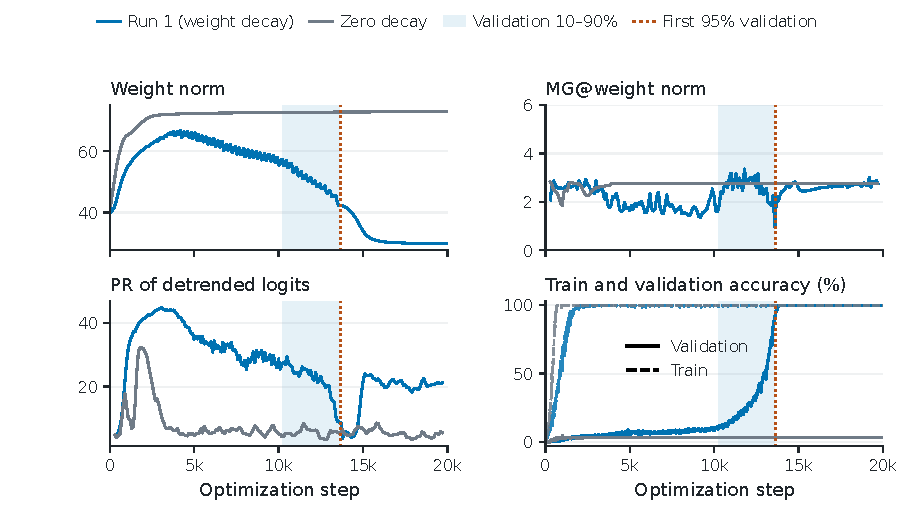
\includegraphics[width=.96\linewidth]{figures/grokking_matched_traces.pdf}
\caption{Two modular-addition runs aligned by optimizer step. MG@weight norm and the covariance PR of detrended logits are shown at window centers. Dashed curves show training accuracy. In run~1, shading spans the sustained validation crossings at 10\% and 90\%. The dotted line marks the first reading at or above 95\%.}
\label{fig:grokking-matched-traces}
\end{figure}

\cx{In the modular-addition example, MG rises as validation accuracy improves and falls, along with logit PR, near the end of the rise. MG also varies in the control while validation accuracy stays low (Figure~\ref{fig:grokking-matched-traces}).}

\cx{The other repeats show why this example needs a comparison. One also has higher MG during the rise than on either side. In the other, median MG is similar during and after the rise, and the gap between training fit and the rise is too short for a complete window (Figure~\ref{fig:grokking-other-runs}).}

\begin{figure}[H]
\centering
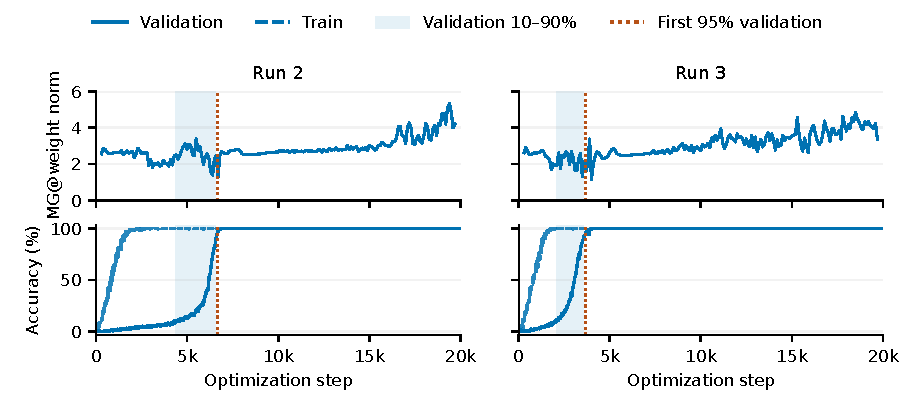
\includegraphics[width=.96\linewidth]{figures/grokking_other_runs.pdf}
\caption{Two further modular-addition runs with weight decay. The time and value scales and the validation markers match Figure~\ref{fig:grokking-matched-traces}.}
\label{fig:grokking-other-runs}
\end{figure}

\cx{Across transformer runs, we locate the rise from sustained crossings of validation accuracy. We compare its median MG with medians from equally long adjacent intervals, using only complete windows after training fit (Table~\ref{tab:grokking-protocol}). A peak during the rise is uncommon and depends on how the rise is defined (Table~\ref{tab:grokking-rise}).}

\begin{table}[!htbp]
\centering\small
\caption{\cx{Runs in which median MG is higher during the rise in validation accuracy than on either side.}}
\label{tab:grokking-rise}
\begin{tabular}{@{}lrr@{}}
\toprule
\cx{Accuracy interval} & \cx{Runs with higher MG} & \cx{Comparable runs} \\
\midrule
\cx{10--90\%} & \cx{2} & \cx{6} \\
\cx{20--80\%} & \cx{1} & \cx{6} \\
\bottomrule
\end{tabular}
\end{table}

\cx{We also test for a brief drop in MG near generalization. We divide the preceding median by the lowest nearby estimate, using matching steps in the controls. All generalizing runs must have a larger ratio than every control for a setting to separate them. Removing the linear trend from the same logs eliminates the separation (Table~\ref{tab:grokking-drop}).}

\begin{table}[H]
\centering\small
\caption{Settings where the MG drop separates grokking runs from controls.}
\label{tab:grokking-drop}
\begin{tabular}{lrr}
\toprule
Weight-norm record & Settings with separation & Usable settings \\
\midrule
Original & 24 & 26 \\
After removing a linear trend & 0 & 26 \\
\bottomrule
\end{tabular}
\end{table}

Covariance PR is also sensitive to drift and correlation time \citep{antognini2018pca}. Roughness changes more than MG. The full-batch perceptron shows no comparable change in MG.

\paragraph{Command smoothing and state repeatability in Walker2d.}
\cx{A Walker2d policy controls the joints of a simulated biped. Starting from a walking policy trained by proximal policy optimization (PPO)} \citep{schulman2017proximal,todorov2012mujoco}, \cx{we continue training with a penalty on changes in successive commands.}

The smoothing objective is
\[
L=L_{\rm PPO}+\frac{\lambda}{6}\mathbb E\|\bar a_\theta(s_{t+1})-\bar a_\theta(s_t)\|_2^2,
\]
\cx{where $\bar a_\theta(s)$ is the mean command vector clipped to $[-1,1]$ per actuator. We average over consecutive steps within episodes and compare MG of the command norm with its value at $\lambda=0$ in the same repeat.}

\cx{Does a more regular record of commands imply a more repeatable stride? In a separate test, both policies start from the same weights and receive the sine and cosine of a prescribed stride phase. We subtract $\lambda(1-\exp[-e_t^2/(2\sigma^2)])$ from the reward, where $e_t^2$ is squared distance to the interpolated state at that phase. We omit horizontal position and rescale velocities when computing the distance (Table~\ref{tab:walker-protocol}).}

\cx{Return error compares the state series with a shifted copy. We use the lag giving the smallest mean squared difference and normalize by twice the total state variance. A second measure asks how much the state varies when each stride returns to the same phase. We divide the variance of the interpolated states at that phase by total state variance. Success requires both measures to improve while reward and completion are preserved (Table~\ref{tab:walker-protocol}). Command smoothing consistently lowers MG, while only some policies trained to follow a prescribed stride meet the state criteria (Table~\ref{tab:walker-motion}).}

\begin{table}[H]
\centering\small
\caption{Command smoothing and state repeatability in Walker2d.}
\label{tab:walker-motion}
\begin{minipage}[t]{.43\linewidth}
\centering
\begin{tabular}{@{}lrr@{}}
\multicolumn{3}{@{}l}{\textbf{Command smoothing}} \\
\toprule
Penalty $\lambda$ & Median MG ratio & Lower MG \\
\midrule
$0.25$ & 0.801 & 5/5 \\
$1$ & 0.604 & 5/5 \\
\bottomrule
\end{tabular}
\end{minipage}\hfill
\begin{minipage}[t]{.51\linewidth}
\centering
\begin{tabular}{@{}lr@{}}
\multicolumn{2}{@{}l}{\textbf{Training with a reference gait}} \\
\toprule
Outcome & Repeats \\
\midrule
State and performance criteria met & 2/5 \\
Lower MG in every reconstruction & 1/5 \\
\bottomrule
\end{tabular}
\end{minipage}
\end{table}

\subsection{Selecting policies for actuator shifts}\label{app:rl_selection}
\cx{Can unperturbed trials identify a policy that retains reward when actuators respond late or noisily? We select among the same candidates using trials with direct actuation, then score their rewards in separate perturbed trials (Table~\ref{tab:walker-protocol}).}

\cx{Candidates must meet the same reward and completion thresholds. If none qualifies, or the fixed choice from the preliminary run is ineligible, the fallback is highest unperturbed reward. Reward includes incomplete episodes. The random rule samples eligible policies uniformly. MG selects the lowest median MG of the command norm over complete episodes. Entropy, normalized squared increments and recurrence use the same scalar record. Increments average squared successive differences divided by twice the variance. Recurrence minimizes the same difference over the lags used in the state-return test (Table~\ref{tab:walker-protocol}). Action smoothness averages squared changes across actuators.}

In the perturbed trials, we compute $v_t=(1-\alpha)u_t+\alpha v_{t-1}+\epsilon_t$ from the current command $u_t$ and the previous filtered value. We start with $v_{-1}=0$ and add independent Gaussian noise of standard deviation $\sigma$ per component. The simulator receives $v_t$ clipped to $[-1,1]$. The recursion retains the unclipped value, including during the initial steps discarded from scoring. Mean reward is the total divided by the planned number of steps, with zero reward after a fall.

\begin{table}[ht]
\centering\small
\caption{Walker2d reward and completion under actuator delay and noise.}
\label{tab:rl_selection}
\begin{tabular}{lrr}
\toprule
Selection rule & Mean reward & Completed episodes \\
\midrule
Spectral entropy & 4.480 & 97.5\% \\
Scalar recurrence & 4.398 & 95.0\% \\
MG (action norm) & 4.313 & 90.8\% \\
Fixed policy choice & 4.310 & 90.8\% \\
Random eligible policy & 4.286 & 90.9\% \\
Highest unperturbed reward & 4.005 & 80.0\% \\
Normalized squared increments & 3.064 & 49.2\% \\
Action smoothness & 2.999 & 47.5\% \\
\addlinespace
Best using perturbed trials & 4.671 & 100.0\% \\
\bottomrule
\end{tabular}

\end{table}

\cx{MG usually improves on selecting by unperturbed reward and gives nearly the same mean reward as the fixed policy. Spectral entropy yields the highest mean reward among rules using unperturbed trials. The final row gives the best eligible choice if perturbed rewards are known (Table~\ref{tab:rl_selection}).}

\section{Timing procedures and information requirements}\label{app:cost}
\cx{We time recording and analysis separately. Direct checks require access to the state update and hidden states for Lyapunov exponents, or to the encoder and decoder for VAE code use.}


\subsection{Timing environments}\label{app:hardware}
The FORCE and forecast timing runs use an Intel Core i5-12500H CPU with one numerical thread. The VAE scheduling test uses two PyTorch threads and one estimator thread. Walker2d timing uses one numerical thread. Hardware metadata are incomplete for the CNN and the VAE scheduling test.



\subsection{Benchmark-specific timing and storage}

\begin{table}[htbp]
\centering\small
\caption{Analysis time on saved records. FORCE times are medians before and after training, in that order.}
\label{tab:cost}
\begin{tabular}{lrlr}
\toprule
Setting & MG & Comparison calculation & Time \\
\midrule
CNN, 1,000-point window & 9.5\,ms & --- & --- \\
FORCE, 256 neurons & 0.835 / 0.598\,s & Full Lyapunov spectrum & 12.006 / 11.551\,s \\
VAE, 512-point window & 12.89\,ms & Mutual information and code swaps & 209.32\,ms \\
\bottomrule
\end{tabular}
\end{table}

\begin{table}[htbp]
\centering\small
\caption{Storage and timing by operation.}
\label{tab:record-cost}
\begin{tabularx}{\linewidth}{@{}p{.20\linewidth}Xl@{}}
\toprule
Experiment & Quantity or operation & Measured cost \\
\midrule
CNN & Store the 32-bit scalar log & 39.06\,KiB \\
& Store the sequence of weight vectors & 559.46\,MiB \\
\addlinespace
FORCE & Simulate and record one neuron before training & 0.102\,s \\
& Simulate and record one neuron after training & 0.166\,s \\
& Largest Lyapunov exponent before training & 0.198\,s \\
& Largest Lyapunov exponent after training & 0.153\,s \\
\addlinespace
Generators & MG on four windows & 8--23\,s \\
& Principal components of all activations & $\sim0.2$\,s \\
\addlinespace
VAE scheduling & One evaluation of loss on fixed sentences & 7.134\,ms \\
& One joint evaluation of MI and decoder sensitivity & 209.323\,ms \\
& All loss evaluations at the primary budget & 51.14\,s \\
& Total estimate with MG at the primary budget & 54.68\,s \\
\addlinespace
Walker2d selection & Actuator command recording without perturbations & 5.52\,s \\
& Trials under actuator delay and noise & 44.7\,s \\
& MG & 0.516\,s \\
& Spectral entropy & 0.00014\,s \\
& Scalar recurrence & 0.0062\,s \\
\bottomrule
\end{tabularx}
\end{table}

\cx{Once the data are recorded, MG is faster than the full Lyapunov spectrum on FORCE states but slower than principal components on generator activations (Tables~\ref{tab:cost} and~\ref{tab:record-cost}).}

\cx{Multiplying each median time by its frequency of use shows that evaluating loss on fixed sentences accounts for most VAE monitoring time. In Walker2d, scalar statistics reuse the recorded commands, while testing gait stability requires further simulations from perturbed states.}



}
